\chapter{Eating Disorder detection}
% deteccion trastornos mentales : dataset, modelos y validacion de los modeloos (resultados)
\label{chap:architecture}
\textit{This chapter presents the methodology used in this work. It describes the overall architecture of the project, with the connections between the different components involved on the development of the project.}

\clearpage
\section{Machine Learning approach}
In order to design the solution we have taken into account the different perspectives that the project could take. To do so, we have decided to first experiment with labelled data in order to perform supervised learning and if we do not achieve good results, we would use other unsupervised learning techniques. In this chapter we are going to talk about the data we have used for this project and the results obtained by using them in Machine Learning models.

In addition, this information has been processed with the objective of optimising the input of the models. This optimisation would take as much data as possible to make the prediction for performing it. Also, we will talk about the procedures carried out with this data.

Furthermore, the data we are going to analyse are texts, so we will have to take this into account for adopting models that use such data. We have mainly focused on the traditional Random Forest, Logistic Regression and SVM models and other more complex pre-trained models such as BERT, specifically using BERT, Mental roBERTa and mBERT.


\subsection{Dataset}
\label{sec:dataset}
% https://arxiv.org/abs/1806.05258
% paper del que se saco
In order to train, validate and then classify and predict, we needed data related to the case study. For this purpose, a search for datasets was made, in which only one labelled dataset related to Eating Disorders have been found. The rest were dataset without labelled data and we wanted to first try the ``Supervised Learning" approach so we decided to continue with the only dataset available. It is the one introduced in~\cite{https://doi.org/10.48550/arxiv.1806.05258} which investigates the creation of high-precision patterns to identify diagnoses of nine mental illnesses and obtains labeled data without having to manually label it.

The dataset, which is called SMHD, was published in conjunction with the paper and is a dataset of social media posts from users with different mental health conditions, including schizophrenia, bipolar disorder, depression, anxiety, obsessive-compulsive disorder, eating disorder, post-traumatic disorder, autism and attention-deficit disorder. In this project we have filtered the data related to Eating Disorders in order to focus on the topic of interest.


% estructura de los datos

For being able to go deeper into the data to be able to use them correctly, an analysis of the information present in the SMHD dataset has been carried out, in order to  adapt the data to ingest them into the Machine Learning model. 

To do this, the type of data and its content have been determined in order to decide which are useful and which can be discarded. Subsequently, all this information will be processed in order to adapt it to our use case. In this use case, as commented before, we want to predict whether a person suffers from Eating Disorder or not by what they write. It should also be noted that, being linguistic and the data being in English, the models have been adjusted to that language, although explorations have been made with other models, as we will discuss in the Section~\ref{sec:models}.

This dataset consists of a set of Reddit posts, concretely 76203 entries of 331 users, labeled with binary classification for suffering an Eating Disorder. In the Table~\ref{tab:SMHDstatistics} there are some useful statistic that have been analysed thoroughly for knowing what we were working with.

\begin{table}[]
\centering
\begin{tabular}{|r|r|r|r|}
\hline
\textbf{}      & \textbf{created\_utc} & \textbf{label} & \textbf{n\_words} \\ \hline
\textbf{count} & 7.620300e+04          & 76203.000000   & 76203.000000      \\ \hline
\textbf{mean}  & 1.441609e+09          & 0.345065       & 161.129457        \\ \hline
\textbf{std}   & 5.741126e+07          & 0.475393       & 282.799671        \\ \hline
\textbf{min}   & 1.209329e+09          & 0.000000       & 0.000000          \\ \hline
\textbf{25\%}  & 1.407560e+09          & 0.000000       & 29.000000         \\ \hline
\textbf{50\%}  & 1.453987e+09          & 0.000000       & 78.000000         \\ \hline
\textbf{75\%}  & 1.490175e+09          & 1.000000       & 184.000000        \\ \hline
\textbf{max}   & 1.514764e+09          & 1.000000       & 12388.000000      \\ \hline
\end{tabular}
\caption{SMHD dataset statistics}
\label{tab:SMHDstatistics}
\end{table}

We can see when the post have been created by using the created\_utc field, which indicates us that the posts were collected around September 2015, being the first post taken from April 2008 and the last one from January 2018. We can determine from this that the time range in which our posts were added to the dataset was wide.

It is interesting to see that in the dataset we have 26295 posts marked as positive and 49908 that are not. That implies that the mean of the label field of the dataset is 0.345065 as we can see in the table. That means that around 34.5\% of the post are classified as positive with a standard deviation of 47.5\% which is close to 50\% and means that our data have enough variation among it. 

The n\_words parameter represents the words per posts that a user has submitted in a certain time. Average posts have 161 words with a standard deviation of 282.8. If we compare the longest post that we have and compare it with the deviation and mean, we incur that there could be outliers.

 We have analyse the contentex in the text using different methods. One of them was using a wordcloud for getting the most used words in the dataset, as you can find in the Figure~\ref{fig:SMHDwordcloud}.

\begin{figure}[!htp]
    \centering
    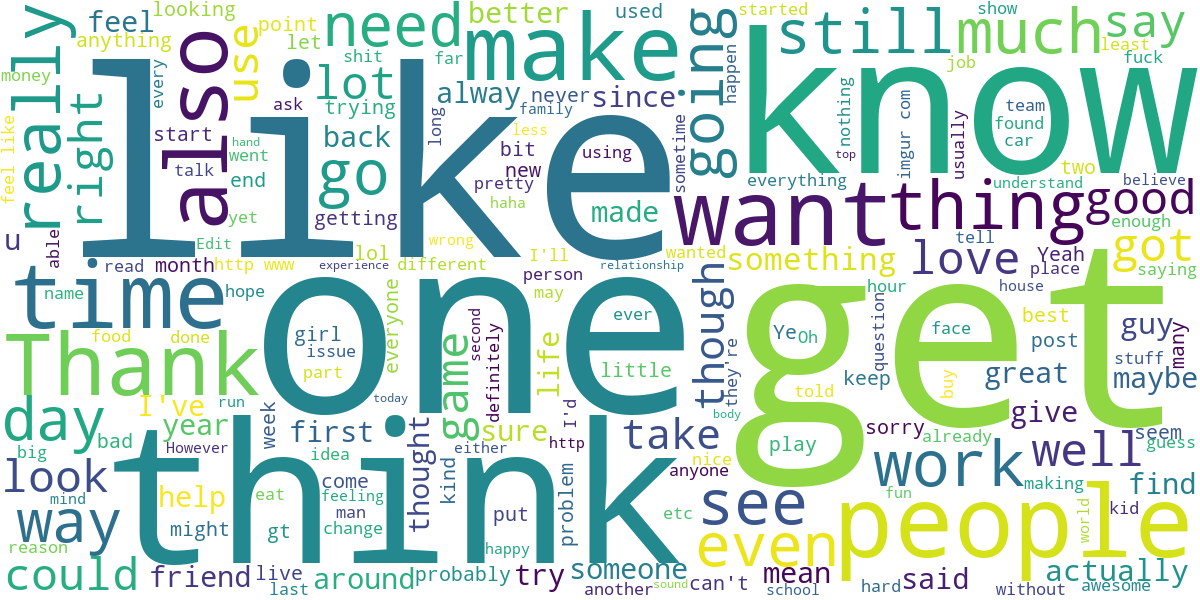
\includegraphics[scale=0.3]{img/detection/SMHD_wordcloud.png}
    \caption{Wordcloud of most common words in SMHD}
    \label{fig:SMHDwordcloud}
\end{figure}

Besides, we have compared the text written by users that are classified as positive from suffering an ED with the ones that are not suffering one. This has been done using scattertext~\cite{JasonKes0:online} that allows us to represent the most frequent and infrequent words from the dataset in a comparing plot as shown in Figure~\ref{fig:scattertext}.

\begin{figure}[!htp]
    \centering
    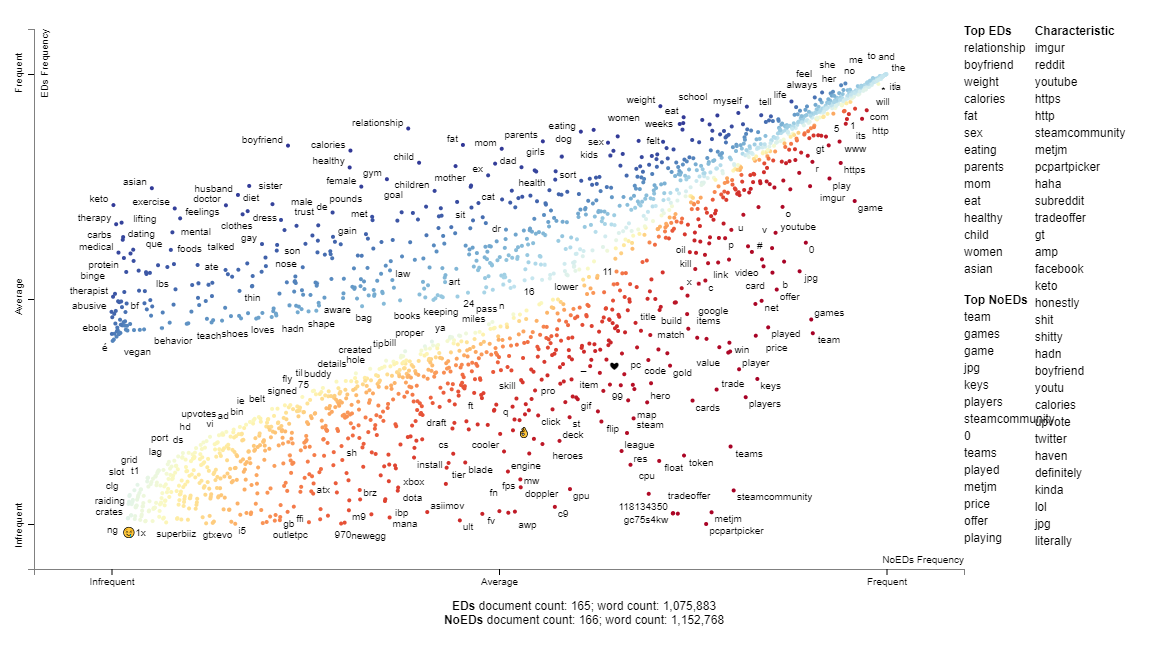
\includegraphics[scale=0.7]{img/detection/scattertext.png}
    \caption{Representation of SMHD dataset with scatter text}
    \label{fig:scattertext}
\end{figure}

As can be seen, the most and least frequent words in the dataset are represented on two axes. The blue colour corresponds to the words published by users who suffer from Eating Disorder and the red ones are those published by people who do not suffer from it. 

Looking at the most frequently used words, interesting conclusions can be drawn, such as that the words most frequently used by users suffering from Eating Disorder are related to health and food, while the most frequent words in the other group are related to games and entertainment. From this we can deduce that the dataset is structured and well focused on our object of study, mental disorders and specifically Eating Disorders.

We can see that the most interesting words to analyse are those that are frequent on one axis of the graph and infrequent on the other, as they are more representative of a specific category. Taking a look at these words gives us a deeper understanding of the data we have.

An analysis of the written main topics has been conducting using also the library scattertext with empath enhancement. Empath is a dictionary that allows to extract several characteristics from the text and its main topic. The results can be seen in the Figure~\ref{fig:empath-scattertext}.

\begin{figure}[!htp]
    \centering
    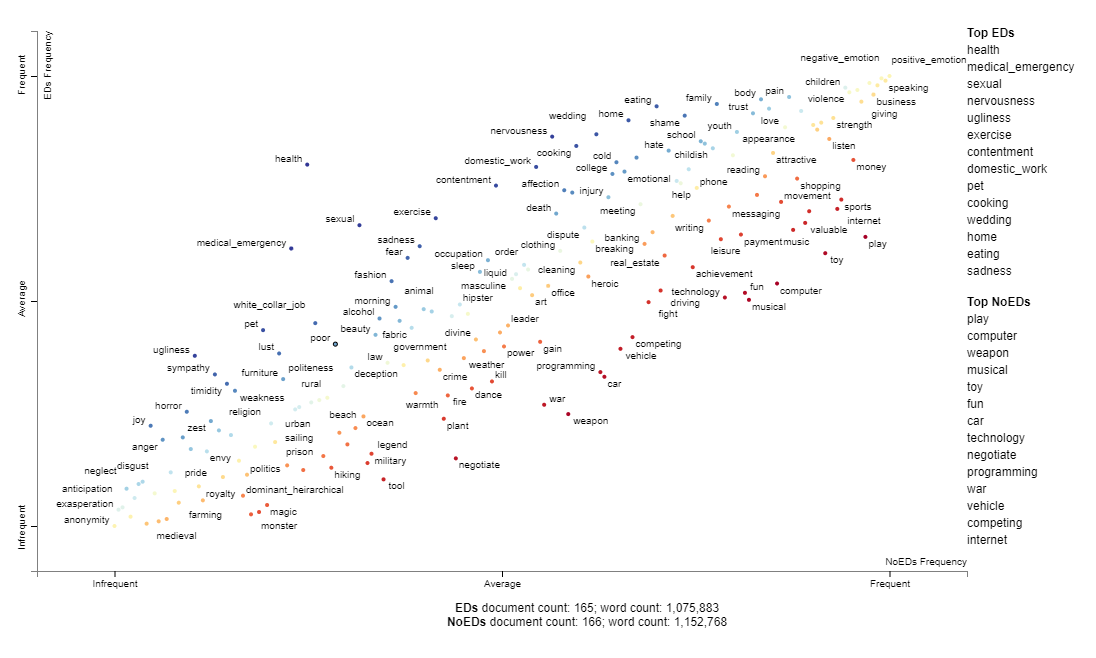
\includegraphics[scale=0.7]{img/detection/empath_scattertext.png}
    \caption{Representation of the topics in SMHD dataset}
    \label{fig:empath-scattertext}
\end{figure}

In this plot we can have a better look on what are the main topics of which the people with and without Eating Disorder talks about. We find that the top five topics of people with Eating Disorder are health, medical emergency, sexual, nervousness and ugliness which are related with having a mental health problem. The top topics for people which don't suffer these problems are mainly related to entertainment, which is expected because the majority of profiles use Social Networks for such.

For a better understanding, these topics are printed taking into account the relation that they have with both categories: they are outliers from one in another. This means that a top topic for people with Eating Disorder is one that is not frequent in the people without it.

After all these different aspects of the dataset have been analysed and understood, we can move on to the pre-processing part, where we adapt all this information for training our model.

\section{Preprocessing}
\label{sec:preprocessing}
Once we had obtained the dataset with which we were going to do the training, we connected to a development environment in order to carry out the pre-processing. We have used the platform of the Jupiter Notebooks department and the Google Collab platform, both of which allow us to create notebooks in which to execute code, specifically Python code, and to have a virtual environment in which to do so.

We load the dataset using Pandas library in the development platform, which allows us to study in depth the characteristics of these as indicated in the Section~ref{sec:dataset} for the information of the SMHD dataset. We can extract different metrics from it, but what we are most interested in is to process the text to put it as input to the model, as it does not work with raw test, but we have to clean it and convert it.

In the Code~\ref{code:preprocessing} we see the treatment given to all the text in the dataset, in which we can see several processes that we are going to explain below.

\begin{lstlisting}[language=Python, caption={Preprocessing function for our data}, label={code:preprocessing}]
def preprocess(words):
    tokens = nltk.word_tokenize(words)
    porter = nltk.PorterStemmer()
    lemmas = [porter.stem(t) for t in tokens]
    stoplist = stopwords.words(`english`)
    lemmas_clean = [w for w in tokens if w not in stoplist]
    punctuation = set(string.punctuation)
    words = [w for w in lemmas_clean if  w not in punctuation]
    return words
\end{lstlisting}

\myparagraph{Tokenization}
Tokenization is a process used to change the text and separate the words of a sentence into an array of words separated by a comma, so that the model understands the input we are providing. For serving this purpose, as seen in the code mentioned above, the word\_tokenize method of the NTLK package has been used.

\myparagraph{Stemmization}
Stemmization is a technique whose aim is to reduce a word to its root or base unit, not necessarily a dictionary-based morphological root, but a part equal to or smaller than the word itself. These are typically rule-based algorithms, which can be seen as a heuristic process that cuts off the end of words. In this, a word is taken through a series of conditionals that determine how to cut it.

An example of this might be English suffixes such as ``-ed" or ``-ing" which do not have much linguistic relevance, being able to relate the words ``play", ``playing" and ``played" which have the same root which is ``play."

The stemming algorithm used in this case is Porter's, which is an algorithm from the 1980s whose aim is to erase the common endings of words so that they can be reduced to a common form. It is not very complex and its development is frozen. It is a good algorithm to start introducing in research branches, as it ensures reproducibility, but it is not recommended for use in a complex application due to its limitations.

\myparagraph{Punctuation and stopwords cleaning}
In order to clean the text, we need to eliminate the part of it that doesn't have any linguistic value like punctuation marks(\textit{e.g.} `.',`!',`?', etc) or stopwords (words, in general adverbs, prepositions, conjunctions and articles, that are meaningless \textit{e.g.} ``the", ``a", ``an", etc.) among others, so we increase the relevance of the remaining items. In order to do so, we take the stopwords provided with the NTLK package and we search for occurences in our text for removing them afterwards.\\


After applying these techniques, we can proceed to pass the data and train the models to fit our data. In the following Section, we will discuss this topic.

\section{Models}
As explained in the previous Section~\ref{sec:studies}, both traditional and newer machine learning methods have been employed. In this section we will look at what they consist of, the techniques used and the statistical results obtained.

In addition, in each model we will analyse the results obtained with them in order to evaluate the optimisation that they may have. To do this, it is necessary to know some statistical measurements that are going to be explained here but before that, we need to understand the basic concepts for making these statistics, which are the possible results from a prediction.
\begin{itemize}
    \item\textbf{ True positive (TP).} True positive is a result that has been predicted as positive and it is correctly predicted.
    \item\textbf{ False positive (FP).} False positive is a result that has been predicted as positive but it is incorrect, it should have been negative. 
    \item \textbf{True negative (TN).} True negative is a result that has been predicted as negative and it is correctly predicted. 
    \item \textbf{False negative (FN).} False negative is a result that has been predicted as negative but it is incorrect, it should have been positive.
\end{itemize}

With these concepts explained, we can dig into the concepts introduced before that we will use for evaluation of the models which are precision, recall, accuracy or F1-score.

\begin{itemize}
    \item \textbf{Precision.} Precision is defined as the number of true positives that have been among all the positive predictions. In an equation it would look like the following.
    \begin{equation}
        precision = \frac{TP}{TP + FP} 
    \end{equation}
    \item \textbf{Recall.} Recall is the measurement of the capacity of the model for classifying true positives.
    \begin{equation}
        recall = \frac{TP}{TP + FN} 
    \end{equation}
    \item \textbf{Accuracy.} Accuracy is the measure of the correct predictions that have been made.
    \begin{equation}
        accuracy = \frac{TP + TN}{TP + FP + TN + FN} 
    \end{equation}
    \item \textbf{F1-score.} F1-score is the mean of precision and recall
    \begin{equation}
        F1-score = \frac{2 * precision * recall}{precision + recall} 
    \end{equation}
    
\end{itemize}

\label{sec:models}
\subsection{Traditional Models}
%% METER ARQUITECTURA MODELS

In this subsection we are going to talk about the models referred to in this project as traditional models, which, as we have said before, are historically more consolidated models.

First of all, we are going to review the architecture that has been followed to implement the different models and has helped us to optimise them. This architecture can be seen in Figure~\ref{fig:mlarchitecture}.


\begin{figure}[!htp]
    \centering
    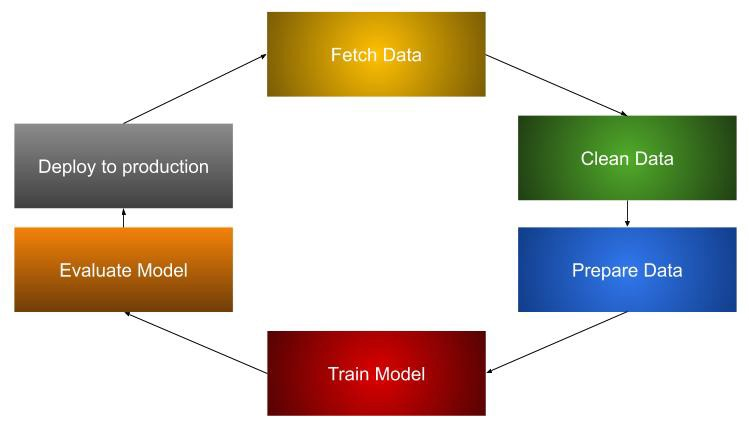
\includegraphics[scale=0.55]{img/detection/mlarchitecture.jpeg}
    \caption{Basic diagram of a Machine Learning architecture}
    \label{fig:mlarchitecture}
\end{figure}

We are going to break down the different steps that are marked in that Figure for explaining what we have done for our traditional models.

\myparagraph{Fetch data}
This part of the architecture is related to data loading. on the training platform. The data described above in~\ref{sec:dataset} are used.

This data is divided into three files, one for training, one for test and one for validation, in JSONL format. We read and load them one by one and using the concatenation that the pandas library allows us to do, we put them together in a single Dataframe object.

\myparagraph{Clean data}
The data coming from the dataset is not always as clean as desired for processing it and it was also our case. We need to clean it up and eliminate the data that is duplicated or not relevant for our case.

This has been performed by a quick exploration to the dataset and the information it contains. Afterwards, we decided which parameters not to use and we deleted them.

\myparagraph{Prepare data}
This procedure is exactly what we have explained in~\ref{sec:preprocessing}. After cleaning, we need to prepare the data in certain format so that the model can process it. 

For doing so, we have applied the line of the Code~\ref{code:apply_preprocessing} in which we apply the preprocess function to all the rows of the Dataframe.

\begin{lstlisting}[language=Python, caption={Preprocessing application}, label={code:apply_preprocessing}]
data[`text`] = data.apply(lambda row: preprocess(row[`text`]), axis=1)
\end{lstlisting}

\myparagraph{Train model}
Once everything is ready and cleaned up, we need to translate the information to a format that the model can understand and be more optimal. This process is called vectorization.

With the vectorization, we achieve better computation times and we make the process of training easier. It consists in extracting features from the text by converting it to numerical vectors.

With this data ready, we can ingest the information to the model. In the first attempt, we don't optimise its hyperparameters and it is after in the evaluation part where we do it.

\myparagraph{Evaluate model}
After getting the results from the first attempt, what we do in our project is to refine the algorithm in order to achieve better results.

There are different libraries that allow to test multiple hyperparameters running the model only once for afterwards checking it. We make use of the GridSearchCV method from the sklearn library, which prompt us after executing it with the better parameters for the model and our data.

We also cross validate the scores obtained using the K-Fold method which consists in an iterative process which divides the data for validating it in a cross way. K groups are made and we train with the k-1 and one of them is used for validating the score. 

\myparagraph{Deploy to production}
If we achieve the results are above a certain minimum of accuracy, we can deploy them to production in order to see them working. 

For doing it, we use a package called pickle that help us to export the model to a file. Our application is a Python server as well as we will explain in Section~\ref{sec:server} so what we need to do in order to deploy it to production is to upload it to this platform.

We need to export the vectorizer as well because it is a particular object that help  us shape our data in the server also.\\

After knowing how this architecture works in our case, we will now focus on the validation and scores obtained when training the models for achieving a final decision on what model we need to use.

\subsubsection{Random Forest}
The model used as explained in Chapter~\ref{chap:state-of-art} is the Random Forest, an algorithm of the sklearn package. We have optimised as much with a number of estimators equal to 400, as well as much as we could with GridSearchCV and we have got the optimised parameters shown in the Table~\ref{tab:RFoptimisedparams}.


\begin{table}[htp]
\centering
\begin{tabular}{|r|r|}
\hline
\textbf{Parameter}  & \textbf{Optimised Value} \\ \hline
max\_depth          & 10                       \\ \hline
min\_samples\_split & 10                       \\ \hline
n\_estimators       & 400                      \\ \hline
random\_state       & 0                        \\ \hline
\end{tabular}
\caption{Optimised parameters for Random Forest}
\label{tab:RFoptimisedparams}
\end{table}

With the use of those parameters we have obtained the scores that can be found in Table~\ref{tab:RandomForestStatistics} that will be discussed at the end of this Chapter.

\begin{table}[htp]
\centering
\begin{tabular}{|l|l|l|l|l|}
\hline
\textbf{}    & \textbf{Precision} & \textbf{Recall} & \textbf{F1-score} & \textbf{Support} \\ \hline
0            & 0.81               & 0.91            & 0.86              & 47               \\ \hline
1            & 0.91               & 0.81            & 0.86              & 53               \\ \hline
accuracy     &                    &                 & 0.86              &  100             \\ \hline
macro avg    & 0.86               & 0.86            & 0.86              & 100              \\ \hline
weighted avg & 0.87               & 0.86            & 0.86              & 100              \\ \hline
\end{tabular}
\caption{Statistics for Random Forest model}
\label{tab:RandomForestStatistics}
\end{table}

\subsubsection{SVM}
We have also used the SVM model for our use case. The configurable hyperparameters of the model have been evaluated by means of a GridSearchCV, in order to optimise it as much as possible to our data. With that procedure we have obtained the parameters seen in Table~\ref{tab:SVMoptimisedparams}.

\begin{table}[h]
\centering
\begin{tabular}{|l|l|}
\hline
\textbf{Parameter} & \textbf{Optimised value} \\ \hline
\textbf{C}         & 100                      \\ \hline
gamma              & 0.01                     \\ \hline
kernel             & rbf                      \\ \hline
\end{tabular}
\caption{Optimised parameters for SVM}
\label{tab:SVMoptimisedparams}
\end{table}

With this hyperparameters we have obtained the statistics shown in Table~\ref{tab:SVM-statistics} which will be discussed in the end of the Chapter.

\begin{table}[!htp]
\centering
\begin{tabular}{|l|l|l|l|l|}
\hline
\textbf{}    & \textbf{Precision} & \textbf{Recall} & \textbf{F1-score} & \textbf{Support} \\ \hline
0            & 0.78               & 0.89            & 0.83     & 47      \\ \hline
1            & 0.89               & 0.77            & 0.83     & 53      \\ \hline
accuracy     &                    &                 & 0.83     & 100     \\ \hline
macro avg    & 0.83               & 0.83            & 0.83     & 100     \\ \hline
weighted avg & 0.84               & 0.83            & 0.83     & 100     \\ \hline
\end{tabular}
\caption{Statistics for SVM model}
\label{tab:SVM-statistics}
\end{table}

\subsubsection{Logistic Regression}
Again, with the Logistic Model regression we proceeded to see which were the best hyperparameters for this model by using GridSearchCV, obtaining the parameters shown in Table~\ref{tab:LRoptimisedparams} obtaining the results shown in Table~\ref{tab:LogisticRegressionStatistics}.

\begin{table}[]
\centering
\begin{tabular}{|l|l|}
\hline
\textbf{Parameter} & \textbf{Optimised value} \\ \hline
C                  & 4.281332398719396        \\ \hline
penalty            & l2                       \\ \hline
solver             & liblinear                \\ \hline
\end{tabular}
\caption{Optimised params for Logistic Regression model}
\label{tab:LRoptimisedparams}
\end{table}

With those we have obtained the statistics of the Table~\ref{tab:LogisticRegressionStatistics} that will be discussed in the following.
\begin{table}[!htp]
\centering
\begin{tabular}{|l|l|l|l|l|}
\hline
\textbf{}    & \textbf{Precision} & \textbf{Recall} & \textbf{F1-score} & \textbf{Support} \\ \hline
0            & 0.80               & 0.91            & 0.85     & 47      \\ \hline
1            & 0.91               & 0.79            & 0.85     & 53      \\ \hline
accuracy     &                    &                 & 0.85     & 100     \\ \hline
macro avg    & 0.85               & 0.85            & 0.85     & 100     \\ \hline
weighted avg & 0.86               & 0.85            & 0.85     & 100     \\ \hline
\end{tabular}
\caption{Statistics for Logistic Regression model}
\label{tab:LogisticRegressionStatistics}
\end{table}


\subsection{BERT Models}
%% METER ARQUITECTURA MODELS
Here we will discuss the BERT models used for making the prediction we want for recognise users with potential of having an Eating Disorder. The architecture of this implementation is much more complex than the one presented before for the traditional models. It is based in Transformers and they have a similar architecture as them, which can be seen in Figure~\cite{fig:BERTarchitecture}.

\begin{figure}[!htp]
    \centering
    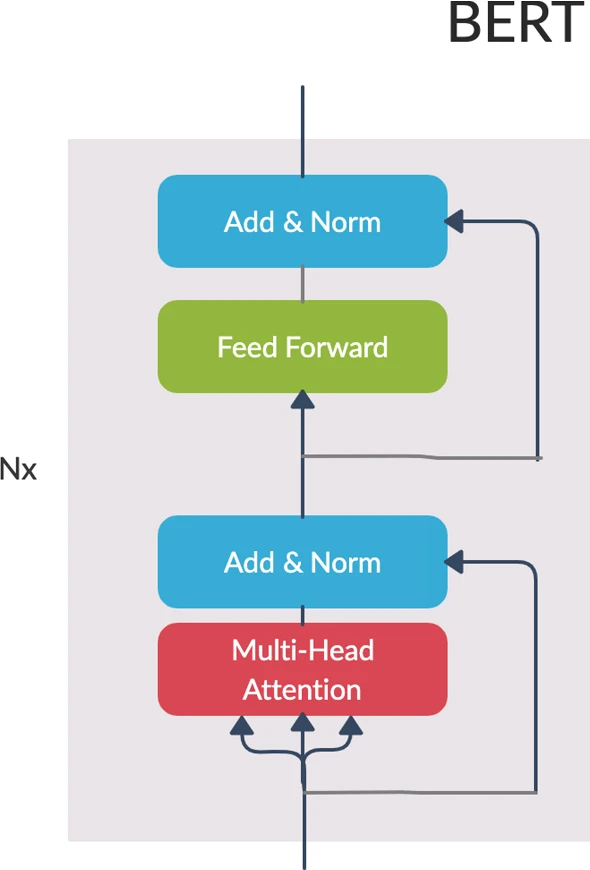
\includegraphics[scale=0.3]{img/detection/bertarchitecture.png}
    \caption{Basic diagram of BERT architecture}
    \label{fig:BERTarchitecture}
\end{figure}

As it can be seen in the Figure, the architecture that is implemented in our models consists of one blocks which is an encoder inherited from the Transformers architecture.

The encoder of the model takes as input a sequence of input words, in our case the words coming from the SMHD dataset. These words are embedded and passed to the positional encoders. Here vectors are assigned to words depending on their positioning in a sentence for extracting the words' contextual meaning. Afterwards, they are passed to the blocks inside the encoder, which are the multi-head attention and a feed-forward network.  

This multi-head attention block, which is a module that runs attention mechanisms in parallel, computes the attention vectors for each input for representing how each word of a specific user of the SMHD dataset is related to the others in the same sentence. Then, it is passed to a feed-forward network, which is on of the simplest type of artificial neural network in which the information moves forward.

One of the pros of using a BERT model is the ability to handle this contextual information from our Eating Disorder dataset. It is because its bi-directional ability; it trains much faster and can be used in applications like ours. There are cons as well, for example that BERT is limited to monolingual classification and the length of input sentences can affect its computation. \\

Now that we are aware of the architecture implemented in our models and its pros and cons, we can move on to discuss the different used BERT models, because we have used variations in order to optimise the statistics of it.


\myparagraph{BERT}
We have implemented the BERT model without any variation, using the bert-based-cased tokenizer and the BERTClassifier model from the Transformers library, and obtained the results shown in Table~\ref{tab:BERTstatistics}.

\begin{table}[!htp]
\centering
\begin{tabular}{|l|l|l|l|}
\hline
Precision & Recall & Accuracy & F1-score  \\ \hline
0.566      & 0.529  &  0.529  & 0.495 \\ \hline
\end{tabular}
\caption{Statistics for BERT model}
\label{tab:BERTstatistics}
\end{table}
The results were not as good as expected so we decided to improve them by using other BERT variants pretrained with specific data that is closer to our case study.

\myparagraph{Mental roBERTa}
This model is pretrained with posts related to mental health problems, which may introduce an improvement in our statistics and the results we obtained were as in Table~\ref{tab:MentalroBERTastatistics}.
\begin{table}[!htp]
\centering
\begin{tabular}{|l|l|l|l|}
\hline
Precision & Recall   & Accuracy & F1-score\\ \hline
0.737      & 0.735   &  0.735   &  0.735      \\ \hline
\end{tabular}
\caption{Statistics for Mental roBERTa model}
\label{tab:MentalroBERTastatistics}
\end{table}

As expected, results were much better using Mental roBERTa but still distant from what we achived with the other models.
\myparagraph{mBERT}
mBERT model is a regular implementation for BERT pretrained with data from more than a 100 languages, so it can provide support for multilingual applications. As it is now, our model only supports text in English but we would like to extend this functionality in the future and this is why we made test with this specific model. The obtained results are as discussed in Table~\ref{tab:mBERTstatistics}.
\begin{table}[!htp]
\centering
\begin{tabular}{|l|l|l|l|}
\hline
Precision & Recall & Accuracy  & F1-score  \\ \hline
0.651      & 0.647 &  0.647    & 0.647 \\ \hline
\end{tabular}
\caption{Statistics for mBERT model}
\label{tab:mBERTstatistics}
\end{table}

And again, as expected the model works much worse than Mental roBERTa as it is not specialized in Mental Health problems but on the other hand, we could win multilanguage support with it. \\

There are more variants that could be implemented such as patentBERT(fine-tuned to perform patent classification), bioBERT (for biomedical text mining) or SciBERT (for scientific texts), but as the results with BERT were not as good as we obtained with the traditional models, we decided to stop working but it is a field from this project that could be investigated for optimising in the future.

And now that we have gathered all the data from the different models, we can discuss what suits better and is more optimised for out application.

\subsection{Discussion}
% exponer las medidas tomadas para cada modelo y dar una valoracion
For clarifying, we are going to summarize the different statistics taken from the different models, for having a clear look of what we have performed so far. They can be seen in the Table~\ref{tab:summarystatistics}.

\begin{table}[h]
\centering
\begin{tabular}{|l|l|l|l|l|}
\hline
\textbf{Model}      & \textbf{Precision} & \textbf{Recall} & \textbf{Accuracy} & \textbf{F-Score} \\ \hline
Random Forest       & 0.86               & 0.86            & 0.86              & 0.86             \\ \hline
SVM                 & 0.83               & 0.83            & 0.83              & 0.83             \\ \hline
Logistic Regression & 0.85               & 0.85            & 0.85              & 0.85             \\ \hline
BERT                & 0.566              & 0.529           & 0.529             & 0.495            \\ \hline
Mental roBERTa      & 0.737              & 0.735           & 0.735             & 0.735            \\ \hline
mBERT               & 0.651              & 0.647           & 0.647             & 0.647            \\ \hline
\end{tabular}
\caption{Summary of the statistics for the different analysed models}
\label{tab:summarystatistics}
\end{table}

This Table throw some light on the analysis performed on the models. We find interesting results which are the following.

\begin{itemize}
    \item The result obtained with the traditional models is good if we take into account that we are working with NLP.
    \item Random Forest and Logistic Regression are the two models that perform better, throwing both results that are similar.
    \item SVM throws good results compared with BERT models but a bit behind from the other two models.
    \item BERT models perform much worse than traditional models.
    \item Regular BERT model performs bad, throwing results close to 50\% which are not acceptable.
    \item Mental roBERTa helps to improve BERT performance but it is not as good as traditional models are.
    \item mBERT provides multilingual support but it has worse performance than Mental roBERTa.
\end{itemize}

From this we can conclude that the models that throw better results are \textbf{Random Forest} and \textbf{Logistic Regression}, which have also a small execution time compared to BERT models. So, we have decided that both of these models can be our main model in our project. We could include mBERT as well for languages that are not English so we will review its viability as well, keeping as principal algorithm the traditional main model.

For refining this decision, we can check the execution times of the models, which will be displayed in the following Table~\ref{tab:timestatistics}.

\begin{table}[h]
\begin{tabular}{|l|l|l|l|l|l|l|}
\hline
\textbf{Model}      & \textbf{Attempt 1} & \textbf{Attempt 2} & \textbf{Attempt 3} & \textbf{Attempt 4} & \textbf{Attempt 5} & \textbf{Mean} \\ \hline
R.F.       & 1.762              & 1.776              & 1.759              & 1.758              & 1.776              & 1.7662             \\ \hline
L.R. & 0.075              & 0.105              & 0.079              & 0.097              & 0.072              & 0.0856             \\ \hline
\end{tabular}
\caption{Execution and mean times of optimised Random Forest and L}
\label{tab:timestatistics}
\end{table}

As it can be seen, Logistic Regression is much faster than Random Forest model. This helps us to determine that \textbf{Linear Regression} is our selected algorith. We can have a performance that is 1\% less in the statistics compared to Random Forest, but the speed of the prediction we gain has much more value for our app. This is because we want to make the system with the user in mind, reducing the complications to use it at minimum.